\documentclass[11pt,a4paper]{article}
\usepackage[spanish,activeacute]{babel}
\decimalpoint
\usepackage[utf8]{inputenc}
\usepackage{listingsutf8}
\usepackage{amsmath}
\usepackage{amsfonts}
\usepackage{amssymb}
\usepackage{graphicx}
\usepackage{color}
\usepackage{listings}
\usepackage{amsthm}
\usepackage{caption}
\usepackage{subcaption}
\usepackage{dsfont}
\usepackage{comment}
\usepackage{enumerate}
\usepackage{enumitem}
\usepackage{mathtools,xparse}
\usepackage{ mathrsfs }
\usepackage{float}
\usepackage{listings}
\usepackage{xcolor}
\usepackage{esvect}
%% CODIGO PYTHON
\definecolor{codegreen}{rgb}{0,0.6,0}
\definecolor{codegray}{rgb}{0.5,0.5,0.5}
\definecolor{codepurple}{rgb}{0.58,0,0.82}
\definecolor{backcolour}{rgb}{0.93,0.93,0.93}

\lstdefinestyle{mystyle}{
    backgroundcolor=\color{backcolour},   
    commentstyle=\color{codegreen},
    keywordstyle=\color{magenta},
    numberstyle=\tiny\color{codegray},
    stringstyle=\color{codepurple},
    basicstyle=\ttfamily\footnotesize,
    breakatwhitespace=false,         
    breaklines=true,                 
    captionpos=b,                    
    keepspaces=true,                 
    numbers=left,                    
    numbersep=5pt,                  
    showspaces=false,                
    showstringspaces=false,
    showtabs=false,                  
    tabsize=2
}

\lstset{style=mystyle, inputencoding=utf8, extendedchars=true, literate={á}{{\'a}}1 {ó}{{\'o}}1 {é}{{\'e}}1 {ú}{{\'u}}1 {í}{{\'i}}1 {ñ}{{\~n}}1,}
%CODIGO PYTHON
\usepackage[left=2.33cm, right=2.31cm, top=2.42cm, bottom=2.42cm]{geometry}
%\renewcommand{\rmdefault}{mathpazo}
%\usepackage{mathpazo}

\usepackage{xcolor}
\usepackage[colorlinks = true,
            linkcolor = blue,
            urlcolor  = blue,
            citecolor = blue,
            anchorcolor = blue]{hyperref}
\hypersetup{
    pdftitle={Proyecto - AA},
    pdfauthor={Mario Muñoz Mesa, Pedro Ramos Suárez},
    pdfsubject={AA},
    pdfkeywords={keyword1, keyword2},
    bookmarksnumbered=true,     
    bookmarksopen=true,         
    bookmarksopenlevel=1,       
    colorlinks=true,   
    linkcolor=black,         
    pdfstartview=Fit,           
    pdfpagemode=UseOutlines,
    pdfpagelayout=TwoPageRight
}


\DeclarePairedDelimiter{\norm}{\lVert}{\rVert}
\NewDocumentCommand{\normL}{ s O{} m }{%
  \IfBooleanTF{#1}{\norm*{#3}}{\norm[#2]{#3}}_{L_2(\Omega)}%
}
\newtheorem{theorem}{Teorema}

\theoremstyle{definition}
\newtheorem{definition}{Definición}[section]


\newtheorem{proposition}{Proposición}[section]


\newtheorem{corolary}{Corolario}[section]


\newtheorem{lema}{Lema}[section]

	\newcommand{\R}{\mathbb{R}}
	\newcommand{\N}{\mathbb{N}}
	\newcommand{\C}{\mathbb{C}}


\title{
\huge \bf Proyecto:\\ Reconocimiento de dígitos manuscritos.\\
	}

\author{Mario Muñoz Mesa\\Pedro Ramos Suárez}
\date{\today}

\begin{document}

	\maketitle
	\renewcommand*\contentsname{Índice}	
	\tableofcontents
	
	\newpage
	
	\section{Descripción y Planteamiento.}
	
	El \href{https://archive.ics.uci.edu/ml/datasets/optical+recognition+of+handwritten+digits}{Dataset Optical Recognition of Handwritten Digits} contiene, con objetivo de reducir dimensionalidad, una transformación de preprocesado en lo que originariamente eran bitmaps $32 \times 32$ de dígitos manuscritos de 0 a 9. En la transformación se divide el bitmap en bloques $4\times 4$ (tendremos 64 bloques) y se asigna a cada uno el número de 1s en el bloque, a cada bloque le corresponderá un entero $n$ con $0\leq n\leq 16$. Ya se nos proporcionan conjuntos de training y test, donde en training se tienen los dígitos dibujados por 30 personas y en test los dibujados por otras 13 personas distintas. El conjunto de training tiene 3823 instancias y el de test 1797 instancias.
	
	\begin{figure}[H]
		\centering
		\begin{subfigure}{.33\textwidth}
  		\centering
 		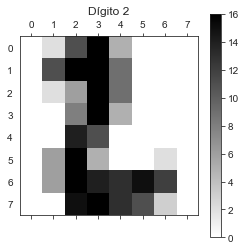
\includegraphics[width=0.9\textwidth]{images/dig2}
  		\label{fig:sub1}
		\end{subfigure}%
		\begin{subfigure}{.33\textwidth}
  		\centering
  		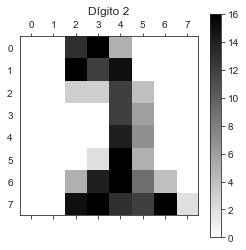
\includegraphics[width=0.9\textwidth]{images/dig22}
  		\label{fig:sub2}
		\end{subfigure}
		\begin{subfigure}{.33\textwidth}
  		\centering
  		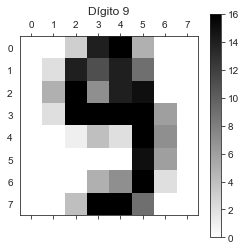
\includegraphics[width=0.9\textwidth]{images/dig9}
  		\label{fig:sub2}
		\end{subfigure}
		\caption{Representación visual de tres de nuestros vectores de características como matriz $8\times 8$, etiquetados como 2, 2 y 9 respectivamente}
		\label{fig:test}
	\end{figure}
	
	Suponemos $(\Omega, \mathcal{A}, P)$ espacio probabilístico, donde $\Omega$ es el conjunto de posibles dígitos manuscritos 0 a 9 en bitmap $32\times 32$ trazados por una persona cualquiera; $\mathcal{A}$ sigma-álgebra formada por todos los subconjuntos de $\Omega$, y $P$ distribución de probabilidad desconocida.
	
	Sobre $(\Omega, \mathcal{A}, P)$ tenemos el vector aleatorio $\mathbf{x}=(x_1,\ldots x_{64})$ donde cada variable aleatoria $x_i\colon \Omega \to \{0,\ldots ,16\}$, $i\in \{1,\ldots,64\}$, mide la cantidad de 1s en el $i$-ésimo bloque $4\times 4$ , y la variable aleatoria $y\colon \Omega \to \{0,\ldots, 9\}$ que asigna el dígito manuscrito. Por lo que $\mathcal{X}=\mathbf{x}(\Omega)=\{0,\ldots ,16\} \times \stackrel{64}{\cdots} \times \{0,\ldots ,16\} = \{0,\ldots ,16\}^{64}$ y $\mathcal{Y}=y(\Omega)=\{0,\ldots,9\}$\\ Buscamos encontrar aproximación de función $f\colon \mathcal{X} \to \mathcal{Y}$ que asigna el dígito correspondiente a cada matriz $8\times 8$ transformada del bitmap original.
	
	Suponemos $(\mathbf{x}_1,y_1),\ldots,(\mathbf{x}_N,y_N)$ con $N=3823$ muestra aleatoria i.i.d (independiente idénticamente distribuida). Lo que se nos ha proporcionado es una realización muestral o dataset $\mathcal{D}=(\mathbf{x}_1,y_1),\ldots,(\mathbf{x}_N,y_N)$ (abuso de notación, ya no son vectores aleatorios). 

	Bajo estas condiciones podemos hacer uso de la Teoría de  Vapnik-Chervonenkis.
	
	\section{Visualización.}
	Podemos visualizar nuestro conjunto de training mediante TSNE (t-Distributed Stochastic Neighbor Embedding)
	%Podemos usar el algoritmo TSNE (t-Distributed Stochastic Neighbor Embedding) para visualizar los datos:
	
	\begin{figure}[H]
	\centering
	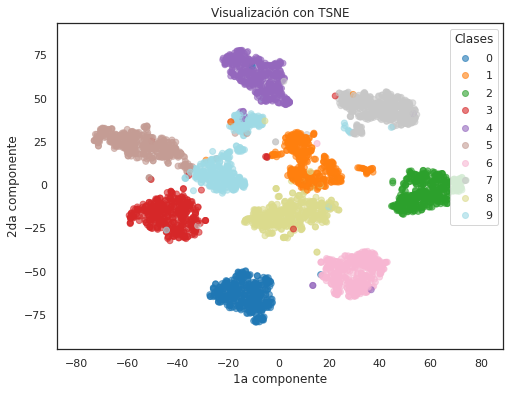
\includegraphics[width=0.5\textwidth]{images/TSNE.png}
	\caption{Visualización de los datos de training mediante TSNE.}
	\end{figure}
	donde observamos agrupamientos por clases, lo cual nos sugiere que obtener un buen clasificador en la muestra es posible.
	%---- añadir último párrafo ya que tenemos i.i.d podemos usar crit ERM que asegura Eout $\to$ 0 cuando Ein $\to$ 0

	
	\section{Hipótesis finales que se usarán.}
	En el preprocesado:
	\begin{enumerate}[label=(\arabic*)]
	\item Se eliminan características varianza menor a 0.05 (también probaremos hipótesis eliminando solo las de varianza 0).
	\item En el caso del modelo lineal se realiza transformación polinomial de segundo orden.
	\item Se normalizan las características (media 0 y varianza 1).
	\end{enumerate}
	
	La métrica a valorar es accuracy. Evaluaremos desempeño de: Regresión Logística multiclase (one vs all), Perceptron Multicapa, Random Forest y Máquina de Soporte de Vectores. Evaluaremos mediante 10-fold cross validation.
	
	\section{Generación de conjuntos training y test. Validación.}
	Hay un compromiso en la selección del tamaño de entrenamiento y test: el tamaño de la muestra de entrenamiento determina el número de instancias que tendremos para entrenar el modelo y por tanto para minimizar $E_{in}$, y el  tamaño del conjunto de test condicionará la estimación, $E_{test}$, de $E_{out}$ que obtengamos. 
	
	En nuestro caso se nos proporciona ya una división en training y test, un 68\% de los datos para training y un 32\% de los datos para test. Cabe mencionar que los datos de test fueron generados por personas distintas a las de training; es por esto que mantendremos la división, esperamos así que $E_{test}$ sea lo más representativo posible de $E_{out}$. En caso contrario (no mantener la división y mezclar para hacer división propia) cabe pensar que el test tiene cierta relación con training, en el sentido de que hay datos generados por misma persona, y las estimaciones en test pudieran ser optimistas.
	
	Para validar sería interesante tener en validación las instancias de vectores de características generadas por autores diferentes a los que generaron el conjunto que estamos entrenando, sin embargo no encontramos información suficiente en la descripción del dataset para proceder así. Utilizaremos $k$-fold cross validation con $k=10$ para la selección de modelos. Esta técnica es derivada de \textit{Leave-one-out}, la cual nos proporciona una estrategia para abordar la problemática o compromiso de elección del tamaño de conjunto de validación, $K$, esta es: $E_{out}(g)\approx E_{out}(g^-)$ cuando $K$ pequeño y $E_{out}(g^-)\approx E_{val}(g^-)$ cuando $K$ grande. %Lo ideal sería utilizar $N$-fold cross validation que equivale a \textit{Leave-one-out}, pero tiene un alto coste computacional.
	
	 La técnica $k$-fold cross validation consiste en dividir la muestra de entrenamiento en $k$ particiones, cada una de tamaño aproximado $\frac{N}{k}$, e ir iterando sobre ellas eligiendo cada vez una partición para actuar como conjunto de validación y entrenando sobre el resto de la muestra el modelo; una vez iteradas sobre todas las particiones se toma la media de errores obtenidos y ese es el error de validación cruzada $E_{cv}\iffalse=\frac{1}{N}\sum_{i=1}^N E_{val}(g_i^-)\fi$ que es un buen estimador de $E_{out}$ cuando $k$ es grande, cuanto menor sea $k$ peor será la estimación de $E_{out}$. Se elige el modelo con menor $E_{cv}$
	 
	  Se podría tomar $k=N$ (Leave One Out) pero esto implica un alto coste computacional; es por esto que se elige $k<< N$, en nuestro caso $k=10$ (es habitual $5\leq k\leq 10$)
	\section{Detalles del preprocesado de datos.}
	Pasos realizados:
	\begin{enumerate}
		%\item Se eliminan las características con varianza 0 pues no aportan información. %Se puede decir que éstas no nos aportan información nueva.
		\item Mostramos visualemente la matriz de coeficientes de correlación lineal habiendo eliminado ya 1 característica que tenía varianza 0 (necesario para poder calcularla)
		\begin{figure}[H]
		\centering
		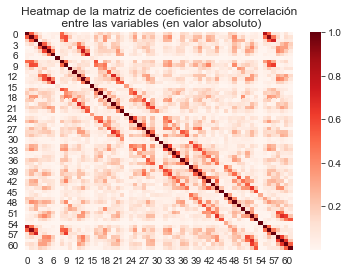
\includegraphics[width=0.5\textwidth]{images/corr_matrix}
		\caption{Matriz coeficientes de correlación lineal.}
		\end{figure}
		No observamos problema de altas correlaciones.
		
		\item Podemos observar las varianzas de las características (todas tienen la misma medida) en training
		
		\begin{figure}[H]
		\centering
		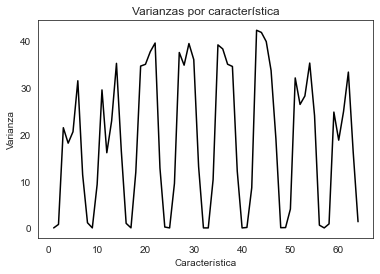
\includegraphics[width=0.45\textwidth]{images/var_caract}
		\caption{Varianzas por característica.}
		\end{figure}
		
		Vemos que hay características con una varianza muy baja. Es por esto que nos planteamos que varias de estas características \iffalse no contribuyen o no están aportando información útil\fi tienen muy bajo poder predictivo. Nuestro caso es fácilmente interpretable y ya podemos intuir que probablemente esquinas o bordes de las imágenes no varíen apenas su valor. %Hay zonas de las imágenes que apenas varían su valor (por ejemplo, puede que las esquinas de las imágenes casi siempre valgan 0).
		
		Eliminaremos las características con varianza menor a 0.05, elegimos un valor prudente. Se eliminan por tanto las características 0, 8, 16, 24, 31, 32, 39, 47 y 56, todas con percentil 99: 0, excepto la 47 que tiene percentil 98: 0, (si nos fijamos todas expresables como $8n$ o $8n-1$ con $n\in \N$, que en la matriz $8\times 8$ corresponden a los bordes laterales)
		%Realizaremos transformación PCA para obtener transformaciones que expliquen el 99\% de varianza acumulada y con la esperanza así de obtener una reducción de dimensionalidad beneficiosa. Elegimos un valor alto de varianza acumulada, tampoco nos interesa perder información (con ese valor ya reducimos a 42 características). Comprobaremos con los resultados sin aplicar PCA para ver si finalmente nos resulta beneficioso o no.
		 \iffalse Elegimos un valor prudente y eliminaremos las características con varianza menor a 0.05
		Las características $7, 8, 10, 11, 19, 20, 21, 22, 23, 31, 32, 34, 35, 43, 44, 46, 47$ tenían valores de coeficiente de correlación mayor a 0.95 en la matriz. Se puede decir que estas características no nos aportan información nueva, además aumentan la dimensionalidad y por tanto empeoran la cota de error de generalización. Se decide eliminarlas y reducir así la complejidad de la clase de funciones. Tras eliminarlas se obtiene
		\begin{figure}[H]
		\centering
		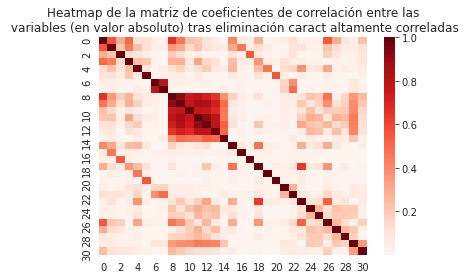
\includegraphics[width=0.62\textwidth]{images/corr_matrix_post}
		\caption{Matriz de coeficientes de correlación en valor absoluto tras la eliminación de características altamente correladas linealmente}
		\end{figure}
		una matriz de menor dimensión y con menor apreciación de zonas correspondientes a alta correlación (excepto en diagonal donde tenemos coeficientes de correlación 1 pues es la correlación de cada característica consigo misma).\fi

		\item En el caso de modelo lineal: Realizamos transformación polinomial de segundo orden a cada característica para aumentar así la flexibilidad de la frontera de decisión de nuestro modelo.
		\item Normalizamos las características (tendrán media 0 y varianza 1), no normalizar puede degradar el desempeño de Gradiente Descendente Estocástico (sensible a la escala de las características), normalización motivada tras la transformación polinómica\iffalse Hay que notar que después de realizar transformación polinomial no tenemos por qué tener características normalizadas\fi . En los casos que no realizamos la transformación polinomial no consideramos que perdamos nada por realizarla aunque nuestras características ya tengan la misma escala. %Volvemos a normalizar las características (que dos variables aleatorias tengan distribución normal no implica que su producto tenga distribución normal)
	\end{enumerate}
	\section{Métrica de error a usar.}
	Visualizaremos el número de vectores de características de la realización muestral pertenecientes a cada clase, esto nos mostrará si hay clases desbalanceadas y qué métrica necesitamos utilizar.
	
	\begin{figure}[H]
		\centering
		\begin{subfigure}{.5\textwidth}
  		\centering
 		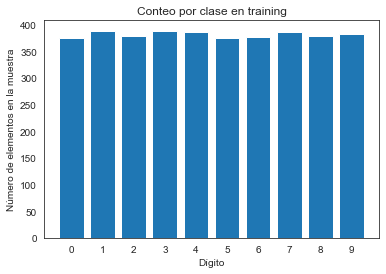
\includegraphics[width=1\textwidth]{images/conteo_por_clase}
  		\label{fig:sub1}
		\end{subfigure}%
		\begin{subfigure}{.5\textwidth}
  		\centering
  		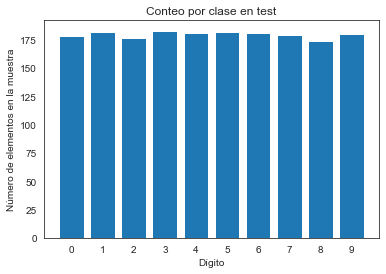
\includegraphics[width=1\textwidth]{images/conteo_por_clase_test}
  		\label{fig:sub2}
		\end{subfigure}
		\caption{Número de elementos por etiqueta de dígito.}
		\label{fig:test}
	\end{figure}
	
	Como podemos ver las clases están balanceadas. Como no tenemos clases desbalanceadas utilizaremos la métrica $accuracy$ que no es más que la proporción de predicciones de clase correctas.
	%$$accuracy:= \frac{TP + TN}{P + N}$$
	%nos da la proporción de predicciones correctas (tanto positivas como negativas). Aquí \textit{TP} denota el número de predicciones positivas correctas, \textit{TN} el número de predicciones negativas correctas, \textit{P} el número verdadero de puntos con etiqueta positiva y \textit{N} el número verdadero de puntos con etiqueta negativa.
	%No necesitamos fijarnos en ninguna métrica especial, basta con minimizar el error en la muestra, conseguir $g$ con el mayor accuracy.\\
	
	\section{Modelo lineal.}
	En el caso del modelo lineal realizaremos una transformación de segundo orden polinomial a los vectores de características, pues aumenta la flexibilidad de nuestra frontera de decisión. \iffalse Para no aumentar en exceso la complejidad de la clase de funciones (mayor dimensión $\Rightarrow$ mayor complejidad $\Rightarrow$ mayor cota de error de generalización) reduciremos previamente la dimensionalidad de nuestros vectores de características (ver parte de preprocesado).\fi No utilizamos transformación polinómica de mayor orden pues cuanto mayor sea la longitud de los vectores de características mayores posibilidades de disminuir el error en la muestra pero mayores posiblidades de aumentar error en la población (sobreajuste); a parte de incrementar el coste computacional.
	
	Por lo que, como hemos comentado, aplicaremos a  $\mathcal{X}$ la transformación $\Phi_2$, que genera combinaciones polinómicas de grado menor o igual a 2 de las características $$\Phi_2(\mathbf{x})=(1,x_1,\ldots, x_{\hat d},\underbrace{x_1x_2,\ldots ,x_1x_{\hat d},x_2x_3,\ldots ,x_2x_{\hat d},  \ldots
	 x_{\hat d-1}x_{\hat d}}_{\text{combinaciones } x_ix_j \text{ con } i<j,\ \  i,j\in \{1,\ldots , \hat d\}}, x_1^2,\ldots x_{\hat d}^2)^T$$
	%Realmente no podemos saber a priori cual es la mejor transformación que podemos hacer, debemos elegir una
	\textit{Nota:} aquí $\hat d< d=64$ pues no utilizaremos todas las características.% Podemos ver que $\Phi_2(\mathbf{x})$ tiene $1+\hat d  + (\sum_{i=1}^{\hat d-1} \hat d -i) + \hat d  = 1 + 2\hat d + (\hat d -1)\hat d - \frac{(\hat d -1)\hat d}{2}=1+2\hat d + \frac{(\hat d -1)\hat d}{2}$ componentes\\
	
	%Dentro de nuestros modelos utilizaremos enfoque probabilístico y determinístico. A continuación se exponen dos técnicas de minimización ya conocidas para enfoque probabilístico y determinístico respectivamente, junto con la clase de funciones hipótesis en cada caso. \\
	%\textit{Nota:} para \texttt{RidgeClassifier} se busca solución analítica de la transformación de nuestro problema de clasificación a uno de regresión, y tendremos $\mathcal{H}:=\{h_w\colon \R^{2\hat d + \frac{(\hat d -1)\hat d}{2}+1}\to \R \ : \ h_w(\Phi_2(\mathbf{x}))=w^T\Phi_2(\mathbf{x}), \ w\in \R^{2\hat d + \frac{(\hat d -1)\hat d}{2}+1}\}$\\
	
	\textbf{Regresión Logística multiclase (One-vs-Rest):} $\quad \quad \quad \quad \quad \quad \quad \quad \quad \quad \quad \quad \quad \quad \quad \quad \quad  $ %(\texttt{SGDClassifier})
	
	Nuestra primera elección es utilizar Regresión Logística multiclase pues en situaciones reales tiene más sentido pensar situaciones probabilísticas que en funciones deterministas. Además la función de error será fácilmente minimizable mediante Gradiente Descendente Estocástico. Asignaremos cada vector de características a la clase que se estime más probable.
	
	Si 
	\begin{itemize}
	\item Tomamos como función objetivo $f\colon \mathcal{X} \to [0,1]^{10}$ con $f(\mathbf{x})=(P(y=0|\mathbf{x}),\ldots, P(y=9|\mathbf{x}))^T$ la función que asigna a cada vector de características el vector de probabilidades de pertenecer a cada clase 
	\item Denotamos con $d$ a $2\hat d + \frac{(\hat d -1)\hat d}{2}$ y con $x$ a $\Phi_2(\mathbf{x})$
	\item Denotamos con $w_i$, $i=1,\ldots , K$, con $K=10$, el hiperplano que separa la clase $i$ del resto
	\end{itemize}
	tenemos la clase de funciones
	%$$\mathcal{H}:=\{h_{w_1,\ldots w_K} \colon \R^{d+1} \to \R^K \ : \ h_{w_1,\ldots w_K} (x)=(\sigma(w_1^T x), \ldots, \sigma(w_K^T x)),\ w_1,\ldots w_K \in \R^{d+1}\}$$
	%$$\mathcal{H}:=\{h_{w_1,\ldots w_K} \colon \R^{d+1} \to \R^K \ : \ h_{w_1,\ldots w_K} (\Phi_2(x))=Softmax((w_1^T \Phi_2(x), \ldots, w_K^T \Phi_2(x))^T),\ w_1,\ldots w_K \in \R^{d+1}\}=$$
	\begin{equation*}
\begin{aligned}
\mathcal{H}= & \Big\{h_{w_1,\ldots w_K} \colon \R^{d+1} \to [0,1]^K \ : \\
      & h_{w_1,\ldots w_K} (x))=Softmax(\ (w_1^T x, \ldots, w_K^T x))^T \ ),\ w_1,\ldots w_K \in \R^{d+1}\Big\}
      \end{aligned}
\end{equation*}
	esto es
      \begin{equation*}
\begin{aligned}
      \mathcal{H}:=& \Big\{h_{w_1,\ldots w_K} \colon \R^{d+1} \to \R^K \ :\\
      & h_{w_1,\ldots w_K} (x)=\frac{1}{\sum_{k=1}^K e^{w_k^T x}}(e^{w_1^T x}, \ldots, e^{w_K^T x})^T,\ w_1,\ldots w_K \in \R^{d+1}\Big\}
\end{aligned}
\end{equation*}
	%$$=\{h_{w_1,\ldots w_K} \colon \R^{d+1} \to \R^K \ : \ h_{w_1,\ldots w_K} (\Phi_2(x))=\frac{1}{\sum_{k=1}^K e^{w_k^T\Phi_2(x)}}(e^{w_1^T \Phi_2(x)}, \ldots, e^{w_K^T \Phi_2(x)})^T,\ w_1,\ldots w_K \in \R^{d+1}\}$$
	
	
	La función de pérdida (máxima verosimilitud) es
	$$E(w_1,\ldots,w_K):=-\ln \left( L(Y|w_1,\ldots ,w_K) \right)=-\sum_{n=1}^N \sum_{k=1}^K y_{nk} \ln \left( \sigma(w_k^T x_n) \right)$$
	donde $\sigma$ es la función logística (sigmoide), $\sigma\colon \R \to [0,1]$, $\sigma(x)=\frac{1}{1+e^{-x}}=\frac{e^x}{e^x+1}$, y $y_{nk} =1$ si $y_n=k$ y $y_{nk}=0$ si $y_n\neq k$\\
	Vemos que
	$$\nabla_{w_j} E(w_1,\ldots,w_K)=\sum_{n=1}^N (\sigma(w_j^T x_n)-y_{nj}) x_n$$
	Utilizaremos SGD (Apéndice 11.1.) para minimizar. Una vez acabada la optimización, obtendremos los $w_1,\ldots ,w_K$ que minimizan $E_{in}$. %Para asignar cada $x\in \mathcal{X}$ a una clase concreta se seguirá el criterio Softmax.
	 Asignaremos entonces cada $x$ a la clase más probable, es decir a la clase $ j'\in \{1,\ldots,K\}$ donde
	 $$j'= \arg max_{j\in \{1,\ldots, K\}} \  \frac{e^{w_j^Tx}}{\sum_{k=1}^K e^{w_k^Tx}}$$
	\subsection{Parámetros usados y tipo de regularización elegida.}
	La regularización nos ayudará a evitar sobreajuste, (en el caso lineal también motivada por la transformación polinómica), con la regularización se aumentará ligeramente el sesgo para decrementar significativamente la varianza. 

	\textbf{Modelo lineal:}	\\
	Utilizaremos regularización Ridge, ahora tendremos error aumentado 
	$$E_{aug}(\mathbf{w})=E_{in}(\mathbf{w})+\lambda \norm{\mathbf{w}}_2^2 = E_{in}(\mathbf{w})+\lambda \mathbf{w}^T\mathbf{w}$$
	donde $\lambda \geq 0$ es el parámetro de regularización. Este tipo de regularización penaliza coeficientes de $\mathbf{w}$ grandes. Otro tipo de regularización conocida es regularización Lasso (utiliza norma $\norm{\cdot}_1$ en lugar de norma $\norm{\cdot}_2$), ésta sin embargo tiende a hacer coeficientes de $\mathbf{w}$ a 0, es buena para selección de características. En nuestro caso consideramos más conveniente Ridge pues confiamos en haber eliminado ya características no informativas en preprocesado.
	%Dos tipos de regularización conocidas son la regularización $l_1$ o Lasso y la regularización $l_2$ o Ridge. La primera es buena para selección de variables, cuando se minimiza hace varios coeficientes 0. La segunda suele dar valores bajos de los coeficientes, penaliza coeficientes altos.
	
	%En nuestro caso se elige regularización Ridge, ya hemos hecho previamente una selección de variables.\\
	
	En Regresión Logística multiclase hemos utilizado la función \texttt{SGDClassifier}, ésta por defecto sigue el criterio one vs rest que ajusta cada clase respecto a las demás, y que es el que utilizaremos por su eficiencia e interpretabilidad. \texttt{SGDClassifier} utiliza tamaño de minibatch 1. Es interesante notar que la función de error junto con el término de regularización Ridge es convexa; pierde relevancia el uso de minibatches o punto de inicio al no tener óptimos locales. Se podría utilizar Gradiente Descendente sin problema. Aún así, dado que \texttt{sklearn} nos proporciona método para la versión estocástica, y que realmente ganamos eficiencia computacional al calcular gradiente en un solo punto, y el ``ruido'' que supone computar el gradiente en un solo punto termina promediándose en número alto de iteraciones; se decide utilizar la versión que nos facilita \texttt{sklearn}.
	
	 El learning rate se ha elegido adaptativo, cuando no se esté mejorando en el criterio de tolerancia tras \texttt{n\_iter\_no\_change} épocas, entonces actualizamos la tasa de aprendizaje mediante $learning\_rate =\frac{learning\_rate}{5}$, vamos disminuyendo conforme nos acercamos al mínimo para prevenir oscilación. Se ha elegido learning rate inicial algo elevado puesto que es adaptativo y  tendremos una tolerancia \texttt{tol} a la que daremos hasta 5 épocas para que se halla disminuido en \texttt{tol} el error. Elegimos hasta \texttt{n\_iter\_no\_change}$=$5 épocas de forma arbitraria, ahora bien, como no sabemos cómo de rápido descenderemos no sabemos qué valor de \texttt{tol} puede ser el adecuado para que tras 5 épocas sin mejora decremente el learning rate, por lo que lo consideraremos como hiperparámetro. El algoritmo parará si llegamos learning rate menor a 1e-6 o por iteraciones máximas. El número de iteraciones se ha elegido arbitrario pero que muestra convergencia, es decir, nuestro algoritmo para por learning rate menor a 1e-6 y no por iteraciones máximas.
	 
	 Se adjunta código con comentarios del resto de parámetros:
	\begin{lstlisting}[language=Python, caption= Par\'ametros usados en SGDClassifier, inputencoding=latin1]
  {"model": [SGDClassifier(
            loss = 'log', # función de pérdida de regresión logística
            penalty = 'l2', # utilizaremos regularización l2 (reg. Ridge)
            # alpha  constante del término de regularización (probaremos distintos valores mediante 10-fold cross validation)
            fit_intercept = True, # añadimos sesgo o intercept pues nuestra matriz aún no tiene columna de 1s 
            max_iter = 180, # Número máximo de iteraciones arbitrario
            #tol  Tolerancia para criterio de parada por tolerancia (parar si loss > best_loss - tol tras n_iter_no_change épocas seguidas)
            # el criterio valora si el error no mejora en tol el mejor error hasta el momento. En nuestro caso esta condición por tolerancia se usará para learning_rate adaptativo
            shuffle = True, # mezclamos después de cada época,
            n_jobs = -1, # máxima paralelización posible en ejecución
            random_state = SEED, # para tener reproducibilidad de los resultados
            learning_rate = 'adaptive', # si no se mejora resultado por criterio tolerancia (loss > best_loss - tol) tras n_iter_no_change épocas seguidas, entonces cambiamos learning rate por (learning rate)/5
                                        # queremos evitar oscilación
            eta0 = 0.05, # learning rate inicial arbitrario
            early_stopping = False, # False pues no queremos reservar más datos para validación, consideramos nuestro dataset pequeño y que no conviene quitar más datos de training
            n_iter_no_change = 5, # cada 5 épocas sin mejora en crit. tolerancia se realizará la adaptación del learning rate (learning_rate='adaptive')
            class_weight = None, # se interpreta que todas las clases tienen peso 1, se elige así pues nuestro problema tiene clases balanceadas
            average = False, # no nos interesa obtener media de pesos
            verbose = 0, # no nos interesan mensajes 
            warm_start = False, # no reutilizamos ninguna solución anterior durante la validación cruzada
            l1_ratio = 0 # 0 corresponde a l2 penalty, no se usará pues solo se usa si learning_rate = 'elasticnet'
            )], # máxima paralelización posible
         "model__alpha": [0.000001, 0.0001, 0.001], # probamos valores de regularización (hiperparámetro)
         "model__tol": [0.0001, 0.001, 0.01]} # probamos distintos valores de tolerancia (hiperparámetro)

	\end{lstlisting}
	
	\section{Perceptron Multicapa.}
	Perceptron Multicapa es una generalización del modelo Perceptron que adquiere una gran flexibilidad pero también potencial sobreajuste, por lo que utilizaremos regularización. En este modelo, la clase de funciones a usar queda determinada por la red. En nuestro caso utilizaremos 3 capas, dos de ellas ocultas y la de salida. La clase de funciones tendrá la forma
	$$\mathcal{H}=\{h_{\mathbf{w}} \colon \R^{d+1} \to [0,1]^{10} \ : \ Softmax \left(\mathbf{w}_3^T \theta (\mathbf{w}_2^T \theta (\mathbf{w}_1^T \mathbf{x}))\right)\}$$
	donde $\theta$ es la función de activación. Ahora la función de pérdida es la función de pérdida de entropía cruzada 
	$$L_{log}(Y,\hat P)=-\log P(Y|\hat P)=-\frac{1}{N} \sum_{i=0}^{N-1}\sum_{k=0}^{K-1} y_{i,k} \log p_{i,k}$$
	donde $K$ es el número de etiquetas, $Y$ es matriz binaria indicadora donde $y_{i,k}=1$ si la instancia $i$ tiene etiqueta $k$, y $\hat P$ es la matriz de probabilidades estimadas con $p_{i,k}=P(y_{i,k}=1)$.
	
	 En Perceptron Multicapa la función  a minimizar no es convexa, la minimización se hará mediante SGD y para el cálculo de gradiente se utilizará el algoritmo Backpropagation. Por la naturaleza de Backpropagation (vamos calculando gradientes desde capa final hasta inicial) tenemos el fenómeno conocido por \textit{Vanishing Gradient Problem}, en nuestro caso no tenemos muchas capas aún así \iffalse para evitar esta problemática\fi podemos elegir función de activación ReLU ($\theta (x)=\max\{0,x\}$) que ayudaría en esta problemática por ser non-saturating function a diferencia de $\tanh$ y $\sigma$ que sí son  saturating functions (ReLU a diferencia de $\tanh$ y $\sigma$ no está acotada superiormente). Con ReLU podemos obtener buenos resultados al igual que con $\tanh$ y $\sigma$, y tendremos ganancia en tiempo de computación. 
	
	Elegiremos método de optimización Adam, tenemos los beneficios de tasa de aprendizaje adaptativa (tasas adaptativas individuales a cada parámetro) y momentum (ayuda a evitar situaciones oscilatorias). Desde scikit-learn vemos que es un método robusto, conocido por dar buenos resultados en datasets de miles de datos como el nuestro, es eficiente y da buenos resultados en validación. Además nos ahorramos tener que hacer tan buena ``afinación'' en los parámetros como en SGD para obtener buenos resultados.
	\subsection{Parámetros usados y tipo de regularización elegida.}
	Utilizaremos regularización Ridge, ahora tendremos error aumentado 
	$$E_{aug}(\mathbf{w})=E_{in}(\mathbf{w})+\lambda \norm{\mathbf{w}}_2^2 = E_{in}(\mathbf{w})+\lambda \mathbf{w}^T\mathbf{w}$$
	donde $\lambda \geq 0$ es el parámetro de regularización. Con este tipo de regularización penalizaremos coeficientes de $\mathbf{w}$ grandes.
	No utilizaremos Early Stopping pues consideramos que no tenemos conjunto de training de gran tamaño y reducirlo más podría degradar los resultados; además cualquier pequeña oscilación en error validación puede hacernos parar antes de tiempo.
	
	\textbf{Estimación de hipérparámetros:}\\
	Para estimar el número de neuronas en las capas ocultas hemos seguido la estrategia de hacer un ``barrido'' inicial  con el mismo número de neuronas en las dos capas ocultas en el rango recomendado (entre 50 y 100) en pasos de 10 en 10, para después hacer un segundo barrido en pasos de 1 en 1 en la zona que muestre mejor accuracy medio en validación cruzada 
	\begin{figure}[H]
		\centering
		\begin{subfigure}{.5\textwidth}
  		\centering
 		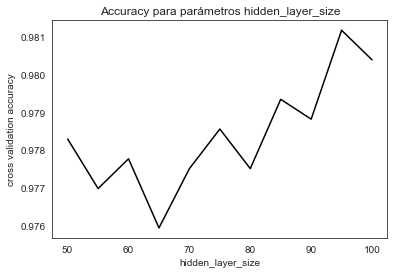
\includegraphics[width=1\textwidth]{images/hidden_layer_est1}
 		\caption{Barrido de 10 en 10 entre 50 y 100}
  		\label{fig:sub1}
		\end{subfigure}%
		\begin{subfigure}{.5\textwidth}
  		\centering
  		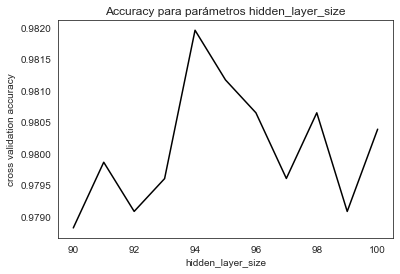
\includegraphics[width=1\textwidth]{images/hidden_layer_est2}
  		\caption{Barrido de 1 en 1 entre 90 y 100}
  		\label{fig:sub2}
		\end{subfigure}
		\caption{Gráficas con accuracy medio por validación cruzada para distintos valores de número de neuronas en ambas capas}
		\label{fig:test}
	\end{figure}
	El mayor valor accuracy medio en validación cruzada lo encontramos con 94 neuronas para ambas capas ocultas, este será el valor elegido.
	
	Como hemos comentado utilizaremos método Adam y función de activación ReLU.
	Una vez fijado el número de neuronas en las dos capas ocultas, tendremos los parámetros:
	\begin{lstlisting}[language=Python, caption= Par\'ametros usados en MLPClassifier, inputencoding=latin1]
  [{"model": [MLPClassifier(
        hidden_layer_sizes=(94,94), # hiperparámetro estimado por validación cruzada
        activation='relu', # elegimos función activación relu por ventajas ante tanh y sigmoide
        solver='adam', # elegimos método adam, robusto y eficiente, no requiere afinar tanto parámetros como sgd
        #alpha parámetro reg. l2 a estimar
        batch_size=128, # elegimos tamaño de batch arbitrario, pensamos que es un tamaño razonable para el tamaño de nuestro dataset aunque no podemos saber cómo se comportará si no es experimentalmente
        # es candidato a hiperparámetro a estimar por cv, nosotros fijamos uno por no hacer cv con mucha carga
        learning_rate='adaptive', # solo usado cuando solver='sgd', no es nuestro caso
        learning_rate_init=0.001, # elegimos learning rate inicial recomendado (pág. 2 https://arxiv.org/pdf/1412.6980.pdf) (buenos resultados por defecto)
        power_t=0.5, # solo usado cuando solver='sgd', no es nuestro caso
        max_iter=250,  # número máximo de épocas arbitrario pero que muestra convergencia
        shuffle=True,  # mezclamos después de cada época
        random_state=SEED, # para tener reproducibilidad de los resultados
        tol=0.001, # tolerancia de parada, si no mejoramos una milésima tras n_iter_no_change épocas entonces paramos, pensamos que es un valor razonable
        verbose=False, # no queremos mensajes
        warm_start=False, # no reutilizamos ninguna solución anterior durante la validación cruzada
        momentum=0.9, # solo usado cuando solver='sgd', no es nuestro caso
        nesterovs_momentum=True, # solo usado cuando solver='sgd', no es nuestro caso
        early_stopping=False, # pues consideramos que tenemos un bajo tamaño de entrenamiento
        validation_fraction=0.1, # no nos importa valor pues no usamos early_stopping
        beta_1=0.9, # elegimos tasa exponential decay para primer momento recomendada (pág. 2 https://arxiv.org/pdf/1412.6980.pdf) (buenos resultados por defecto)
        beta_2=0.999, # elegimos tasa exponential decay para segundo momento recomendada (pág. 2 https://arxiv.org/pdf/1412.6980.pdf) (buenos resultados por defecto)
        epsilon=1e-08, # valor numerical stability para adam recomendado (pág. 2 https://arxiv.org/pdf/1412.6980.pdf) (buenos resultados por defecto)
        n_iter_no_change=10, # damos hasta 10 épocas para mejorar error en 0.001, si no se mejora pararemos
        max_fun=15000)], # solo usado cuando solver='lbfgs', no es nuestro caso
        "model__alpha": [0.00001,0.0001,0.001]} # parámetro de reg. l2 para cross validation

	\end{lstlisting}
	\section{Máquina de Soporte de Vectores.}
	Elegimos SVM porque contempla una posibilidad que no contempla ninguno de los otros modelos, que es buscar solución con ``margen amplio'', por lo que la dimensión $d_{VC}$ de nuestra solución será menor y podemos esperar más capacidad de generalización.\\ SVM persigue buscar un hiperplano frontera de clasificación óptimo, óptimo en el sentido de maximizar su distancia a los puntos frontera de cada clase (vectores soporte) (buscamos ``pasillo'' lo más ancho posible), éste se resuelve como problema programación cuadrática con  restricciones. Cuando los datos no son separables en espacio original pero al transformarlos sí, entonces programación cuadrática con restricciones ofrece solución pero una eficiencia inabordable. En este caso resolvemos el problema dual utilizando el ``truco del kernel'' (nos facilita el cálculo del producto escalar de transformación de vectores). El problema hasta ahora se conoce como Hard-Margin SVM.
	
	Nosotros usaremos la versión ``suave'', Soft-Margin SVM, pues pretendemos evitar incurrir en sobreajuste por ruido al introducir un margen de violabilidad del pasillo para cada punto. \iffalse $\xi \geq 0$ para cada punto $(\mathbf{x}_n, y_n)$. El problema consiste ahora en encontrar
	$$\min_{b,\mathbf{w},\mathbf{\xi}} \frac{1}{2} \mathbf{w}^T \mathbf{w} + C\sum_{n=1}^N \xi_n \text{verificando}\begin{cases} y_n(\mathbf{w}^T \mathbf{x}_n + b) \geq 1-\xi_n \\ \xi_n\geq 0 \end{cases} \forall n \in \{1,\ldots,N\}$$\fi
	Finalmente la función a minimizar es
	$$ \min_{\mathbf{c},\mathbf{w}} \lambda \mathbf{w}^T\mathbf{w} + \underbrace{\frac{1}{N}\sum_{n=1}^N \max\{1-y_n(\mathbf{w}^T\mathbf{x}_n+b),0\}}_{E_{SVM}(b,\mathbf{w})} \quad \lambda=1/2CN$$
	Elegimos kernel RBF pues en principio no tiene por qué darnos peor resultado que el kernel polinomial, y nos facilita el ajuste al tener solo un parámetro $\lambda$ para ``afinar''.
	
	
	\subsection{Estimación de hiperparámetros.}
	Tendremos dos hipérparámetros a estimar $\gamma$ y $C$.	Para valores $C$ grandes tendremos baja violabilidad del pasillo (pasillo estrecho), y con $C$ pequeño más libertad de violabilidad. Por otra parte tenemos el parámetro $\gamma$ asociado a nuestro kernel que determinará cómo de lejos puede cada punto influir en la determinación de la frontera de decisión; actúa como la inversa del radio de influencia (valores bajos: lejos, valores altos: cerca).
	
	Desde la documentación de scikit-learn se nos indica que un grid de búsqueda en escala logarítmica entre $10^{-3}$ y $10^3$ suele ser suficiente para estimar $C$ y $\gamma$.
	La estrategia que hemos seguido ha sido tomar 7 parámetros para $C$ entre $10^{-3}$ y $10^3$ siguiendo escala logarítmica, y para cada uno hacer una búsqueda dicotómica de $\gamma$ (binaria, desplazándonos hacia los valores que dan más accuracy). El parámetro $C$ ganador fue 10 
	\begin{figure}[H]
		\centering
		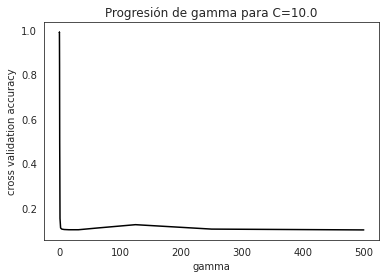
\includegraphics[width=0.45\textwidth]{images/prog_gamma}
		\caption{Progresión de $\gamma$ para $C=10$ (de derecha a izquierda)}
		\end{figure}
	y el ganador $\gamma$ junto a ese $C$ fue $\gamma =0.02007346725463867$\\
    Adjuntamos código con el resto de parámetros
    \begin{lstlisting}[language=Python, caption= Par\'ametros usados en SVC, inputencoding=latin1]
  {"model": [SVC(C=w_p_c, # hiperparámetro estimado c, w_p_c=10
        kernel='rbf', # kernel Radial Basis Function
        degree=3, # solo para kernel poly, no es nuestro caso
        gamma=w_p_gam, # hiperparámetro estimado gamma, w_p_gam=0.02007346725463867
        coef0=0.0, # solo para kernel poly, no es nuestro caso
        shrinking=True, # suponemos número alto de iteraciones, nos podrá ayudar a reducir tiempo de cómputo
        probability=False, # consideramos que no es necesario y nos aumentaría coste computacional
        tol=0.001, # tolerancia para criterio parada, hasta milésima
        cache_size=200, # puede mejorar tiempo ejecución para problemas de muchos datos, en nuestro caso consideramos que son pocos datos y que con 200MB sería suficiente
        class_weight=None, # suponemos todas las clases con peso 1 pues tenemos clases balanceadas
        verbose=False, # no queremos mensajes
        max_iter=-1, # no establecemos criterio de parada por iteraciones
        decision_function_shape='ovr', # devolvemos función decisión one vs rest 
        break_ties=False, # no consideramos casos de empates, y ahorraremos considerablemente en coste computacional
        random_state=SEED)], # para tener reproducibilidad de resultados
        }

	\end{lstlisting}
	\section{Random Forest.}
	El modelo Random Forest consiste en crear una serie de árboles, utilizando $\textit{bootstrap}$ y fijando el número de características de cada árbol a la raíz del número total de características, seleccionadas de manera aleatoria.
	
	La función de pérdida que intentamos minimizar es:
	$$C_{\alpha}(T) = \sum_{m=1}^{|T|} N_{m} Q_{m}(T) + \alpha |T|$$
	donde $|T|$ es el número de nodos terminales, $\alpha$ es el parámetro de complejidad utilizado para la poda de costo mínimo-complejidad, $N_{m}$ es el número de muestras que hay en el nodo $m$, y $Q_{m}(T)$ es la medida de la impureza de los nodo $m$.
	
	Como medida de la impureza $Q_{m}$ utilizaremos el criterio de impurezas Gini Index, que viene dada por:
	$$Q_{m}(T) = \sum_{k=1}^{K} \hat{p}_{mk} (1 - \hat{p}_{mk})$$
	donde $\hat{p}_{mk}$ es la proporción de la clase $k$ en el nodo $m$, y viene dada por:
	$$\hat{p}_{mk} = \frac{1}{N_{m}} \sum_{x_{i} \in R_{m}} [y_{i} = k]$$
	donde $R_{m}$ es la región que representa el nodo $m$. \\
	Utilizamos el criterio Gini Index en lugar de entropy porque los resultados son similares y nos ofrece mejor eficiencia al no tener que computar función logarítmica.
	
	El número de árboles será hiperparámetro y para estimarlo utilizaremos $\alpha =0$
	%Para la selección de hiperparámetros utilizaremos $\alpha = 0$, por lo que nos quedará:
	%$$C_{\alpha}(T) = \sum_{m=1}^{|T|} N_{m} Q_{m}(T)$$
	
	\subsection{Estimación de hipérparámetros:}
	
	Para estimar el número de árboles de decisión utilizados, utilizamos de nuevo la estrategia de hacer un ``barrido'' inicial con el número de árboles entre 50 y 500 en pasos de 50 en 50, para luego hacer más barridos reduciendo el tamaño del intervalo y de los pasos hasta encontrar un buen valor.
	
	\begin{figure}[H]
		\centering
		\begin{subfigure}{.45\textwidth}
  		\centering
 		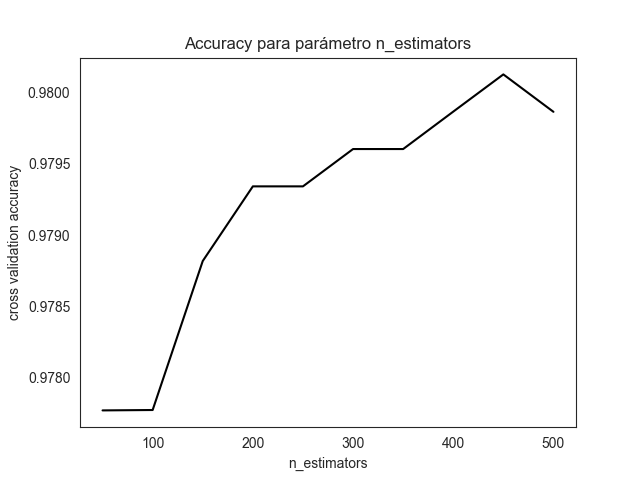
\includegraphics[width=1\textwidth]{images/n_est1}
 		\caption{Barrido de 50 en 50 entre 50 y 500}
  		\label{fig:sub1}
		\end{subfigure}
		\begin{subfigure}{.45\textwidth}
  		\centering
  		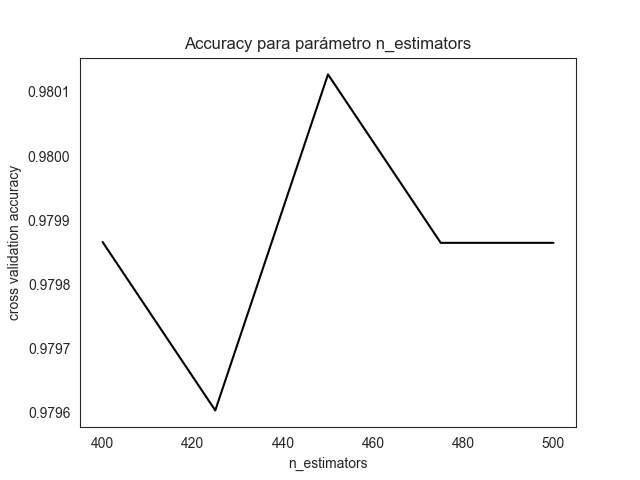
\includegraphics[width=1\textwidth]{images/n_est2}
  		\caption{Barrido de 25 en 25 entre 400 y 500}
  		\label{fig:sub2}
		\end{subfigure}
		\begin{subfigure}{.45\textwidth}
  		\centering
 		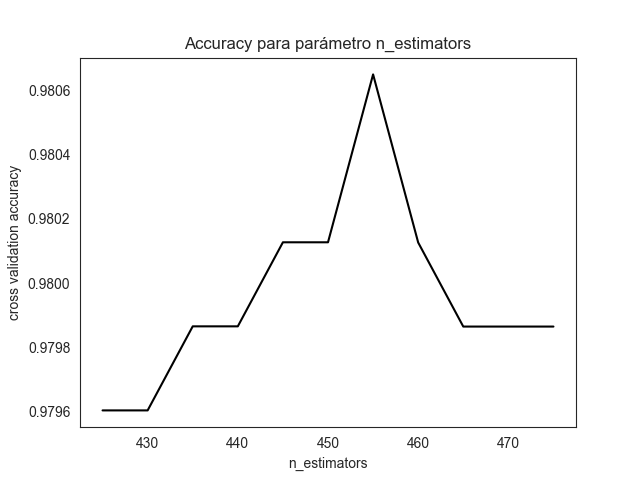
\includegraphics[width=1\textwidth]{images/n_est3}
 		\caption{Barrido de 5 en 5 entre 425 y 475}
  		\label{fig:sub3}
		\end{subfigure}
		\begin{subfigure}{.45\textwidth}
  		\centering
  		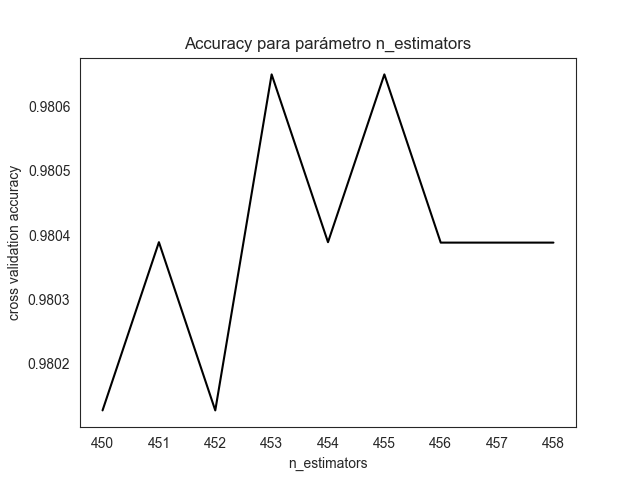
\includegraphics[width=1\textwidth]{images/n_est4}
  		\caption{Barrido de 1 en 1 entre 450 y 458}
  		\label{fig:sub4}
		\end{subfigure}
		\caption{Gráficas con accuracy medio por validación cruzada para distintas cantidades de árboles de decisión.}
		\label{fig:test}
	\end{figure}
		
		El mayor valor de accuracy lo obtenemos para 453 y 455 árboles de decisión, por lo que usaremos 453 árboles para que el tiempo de ejecución sea ligeramente inferior al tener menos árboles.
		
		Utilizando el criterio Gini Index como hemos comentado previamente, y 453 árboles de decisión, los parámetros finales para el modelo son:
		
			\begin{lstlisting}[language=Python, caption= Par\'ametros usados en RandomForestClassifier, inputencoding=latin1]
  {"model": [RandomForestClassifier(
        n_estimators=453,   # usamos el número de estimadores calculados
        criterion='gini',   # usamos gini porque es mas rapido y nos da resultados similares
        max_depth=None,     # para que explore la profundidad maxima del arbol
        min_samples_split=2,  # número mínimo de muestras para dividir un nodo, con 2 divide siempre que no sean hojas
        min_samples_leaf=1,     # una hoja se considera cuando solo es una muestra
        min_weight_fraction_leaf=0.0,   # para que todas las hojas tenga el mismo peso
        max_features='auto',    # utiliza la raiz cuadrada del número de características
        max_leaf_nodes=None,    # para que utilice todos los arboles
        min_impurity_decrease=0.0,  # para que expanda todos los nodos
        min_impurity_split=None,    # para que expanda todos los nodos
        bootstrap=True,     # como hemos visto en teoría, mejoramos los resultados usando bootstrap
        oob_score=True,     # solo queremos que use los datos de la muestra
        n_jobs=-1,      # para que utilice todos los cores del procesador
        random_state=SEED,  # para tener reproducibilidad de los resultados
        verbose=0,  # no queremos mensajes
        warm_start=False,   # para que cree el arbol de cero
        class_weight=None,  # para que todas las clases tengan el mismo peso
        #ccp_alpha grado de penalización por complejidad. Cuanto más alto más podado. Parámetro para regularizar y evitar sobreajuste. Será hiperparámetro a estimar
        max_samples=None)], # para que utilize todos los datos
        "model__ccp_alpha": [0.0, 1e-1, 1e-2, 1e-3, 1e-4, 1e-5]} #hiperparámetro a estimar

	\end{lstlisting}
	
	
	\section{Selección del mejor modelo.}
	Para la selección del mejor modelo utilizamos 10-fold cross validation como ya comentamos. Elegiremos como modelo ganador aquel con menor $E_{cv}$. El modelo ganador se entrenará finalmente sobre toda la muestra. Para hacer esto utilizamos \texttt{GridSearchCV}, función que nos permite entrenar el modelo ganador en toda la muestra mediante \texttt{refit=True}, y nos facilita variables con los resultados obtenidos. La métrica considerada para la elección del mejor modelo es el accuracy (tenemos clases balanceadas).
	
	Las funciones de los modelos con parámetros ganadores son 
	\begin{itemize}
		\item \texttt{SGDClassifier(eta0=0.05, l1\_ratio=0, learning\_rate='adaptive', loss='log',\\ max\_iter=180, tol=0.0001, alpha=0.0001)}
		\item \texttt{MLPClassifier(alpha=1e-05, batch\_size=128, hidden\_layer\_sizes=(94,94),\\ learning\_rate='adaptive', max\_iter=250, tol=0.001)}
		\item \texttt{RandomForestClassifier(ccp\_alpha=0.0, n\_estimators=453)}
		\item \texttt{SVC(C=10, gamma=0.02007346725463867)}
	\end{itemize}
	Nos referiremos a estos modelos, con los parámetros ya comentados, como $M_{RLClass}$, $M_{MLPClass}$ y $M_{RandForestClass}$ y $M_{SVMClass}$ respectivamente. Veamos los accuracies medios obtenidos con 10-fold cross validation

	\begin{table}[H]
	\begin{center}
	\begin{tabular}{|c|c|c|}
	\hline
	 Modelo & Accuracy medio 10-fold cross validation \\
	\hline \hline
	$M_{SVMClass}$ & 0.98979878 \\ \hline
	$M_{SGDClass}$ & 0.98325906\\ \hline
	$M_{MLPClass}$ & 0.98195563 \\ \hline
	$M_{RandForestClass}$ & 0.98065014  \\ \hline
	\end{tabular}
	\caption{Accuracies medios por 10-fold cross validation de cada modelo.}
	\label{tabla:sencilla}
	\end{center}
	\end{table}
	Elegimos el modelo con menor $E_{cv}$, en este caso $M_{SVMClass}$ (mayor accuracy). Una vez nuestro modelo ganador es entrenado sobre toda la muestra de entrenamiento (en 10-fold cross validation no utilizábamos $N$ instancias, siempre reservábamos una de las 10 particiones para validar), utilizaremos nuestro conjunto de test que guardamos desde el principio para estimar el error de generalización, estimaremos $E_{out}$ mediante $E_{test}$. Procediendo así, y teniendo en cuenta que estamos valorando mediante la métrica accuracy, estimamos error, de muestro mejor modelo $M_{SVMClass}$, fuera de la muestra: $1-0.97495826 = 0.02504174$. Podemos observar que es un error algo más elevado que el obtenido por validación cruzada $1-0.98979878 = 0.01020122$, aquí es donde juega su papel como medida de calidad el haber mantenido en test las imágenes de autores diferentes a los implicados en training (podríamos decir que al no ser los mismos autores no hemos ``modelado la forma de escritura propia de los autores'', hay un ``comportamiento'' en test no modelado; la idea es que sea así por los motivos ya explicados en el punto 4).\\
	
	Mostramos:
	\begin{itemize}
	\item  La matriz de confusión del modelo ganador:
	\begin{figure}[H]
	\centering
	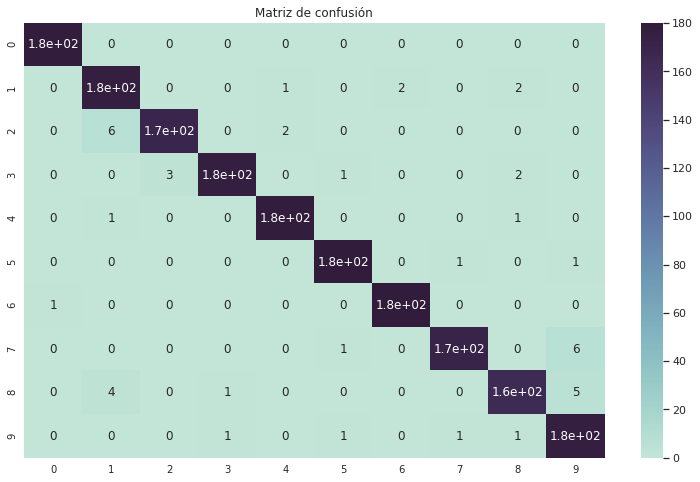
\includegraphics[width=0.55\textwidth]{images/confusion}
	\caption{Matriz de confusión de $M_{SVMClass}$ para test.}
	\end{figure}
	La matriz de confusión nos muestra las etiquetas predichas (eje x) y las verdaderas (eje y). Observamos que la mayoría de datos se encuentran en la diagonal, lo cual nos asegura que nuestro modelo realiza una buena clasificación.\\

	\item Y la curva de aprendizaje del modelo ganador 
	\begin{figure}[H]
	\centering
	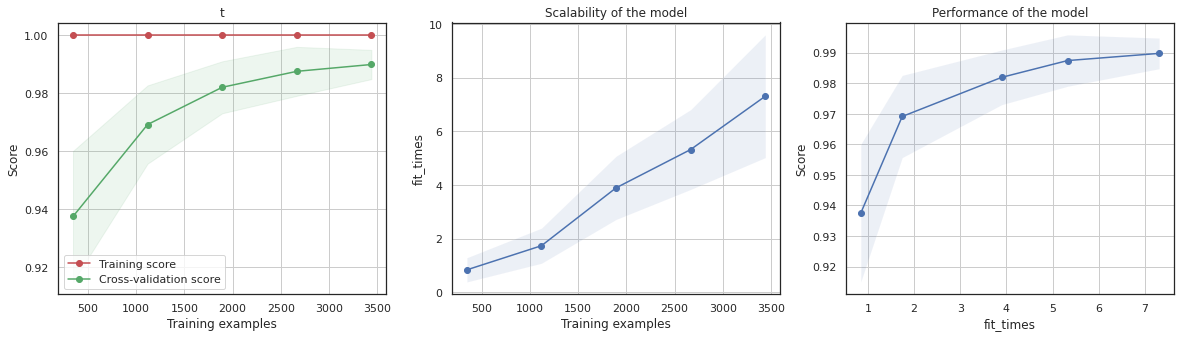
\includegraphics[width=1\textwidth]{images/learning_curve}
	\caption{Curva aprendizaje, escalabilidad y desempeño del modelo ganador $M_{SVMClass}$. (código para la generación de la gráfica tomado de \url{https://scikit-learn.org/stable/auto_examples/model_selection/plot_learning_curve.html})}
	\end{figure}
	en la que observamos que: (1) nuestro modelo consigue constantemente clasificar muy bien el conjunto de entrenamiento, (2) el accuracy en validación cruzada asciende en forma logarítmica conforme aumenta el conjunto de entrenamiento, cuanto mayor sea la muestra de entrenamiento más se aprende. Por otra parte, en la escalabilidad del modelo, vemos que cuantas más muestras de entrenamiento más tiempo en ajustar, asciende de forma lineal por lo cual consideramos que no tiene una muy mala escalabilidad. En el desempeño del modelo podemos observar que cuanto más tiempo de ajuste mayor accuracy pero las mejoras cada vez son menores.
	\end{itemize}
	
    % En libro Learning from data no encuentro nada de esa forma de cota. En sección 2.2.3 habla cota mediante % test pero usa |H|=1 porque solo hay una hipótesis que es la g de H, ¿viene en los apuntes o libro la fórmula que pusiste tú?
	Además, podemos dar una cota de $E_{out}$ basada en $E_{test}$ mediante la desigualdad de Hoeffding. Ahora ya tenemos 1 función hipótesis ganadora fijada $\mathcal{H}=|\{g\}|=1$, por lo que, tomando $\delta=0.05$ y valorando métrica accuracy
	$$E_{out}(g) \leq \underbrace{0.02504174}_{E_{test}(g)}+\sqrt{\frac{1}{2\cdot 1797} \log \left(\frac{2}{0.05}\right)} \quad \textit{ con probabilidad } \geq 1-0.05$$
	esto es, tenemos que $E_{out}(g)\leq 0.04615475961$ con probabilidad $\geq 0.95$.\\
    %$$E_{out}(g) \leq E_{test}(g) + \sqrt{\frac{1}{2N_{test}} \log \(\frac{2 |\mathscr{H}|}{\delta}\)} \quad \text{con probabilidad} \geq 1 - \delta$$
    %donde $N_{test}$ es el número de mustras en el conjunt $\textit{test}$, y $|\mathscr{H}|$ es el número de modelos comparados. \\
    %Fijando un valor de $\delta$, por ejemplo $\delta = 0.05$, y utilizando la fórmula anterior:
    %$$E_{out}(g) \leq 0.02726767 + \sqrt{\frac{1}{2 \cdot 1797} \log \frac{2\cdot 4}{0.05}} \approx 0.06484591$$
    %es decir $E_{out}(g)\leq 0.06484591$ con probabilidad mayor o igual a $0.95$
    %podemos garantizar con un $95\%$ de certeza de que el error fuera de la muestra es menor que un $6\%$.
    
    Podemos comprobar que se tomó la función hipótesis con menor error estimado fuera de la muestra viendo el desempeño de los otros modelos en test
	\begin{table}[H]
	\begin{center}
	\begin{tabular}{|c|c|c|}
	\hline
	 Modelo & Accuracy en test & Accuracy en entrenamiento \\
	\hline \hline
	$M_{SVMClass}$ & 0.97495826 & 1 \\ \hline
	$M_{SGDClass}$ & 0.97273233 & 1\\ \hline
	$M_{MLPClass}$ & 0.96382860 & 1 \\ \hline
	$M_{RandForestClass}$ & 0.97161937 & 1  \\ \hline
	Aleatorio & 0.10294936004451864 & 0.09285901124771122 \\ \hline
	\end{tabular}
	\caption{Accuracies en entrenamiento y test de los modelos una vez entrenados sobre toda la muestra de entrenamiento. Añadimos accuracy de modelo aleatorio, se aprecia diferencia sustancial.}
	\label{tabla:sencilla}
	\end{center}
	\end{table}
	Comprobamos que $M_{SVMClass}$ es el que mejor accuracy tiene en nuestra estimación fuera de la muestra (en test).\\
	~\\
	
	Por último cabe mencionar que se realizó todo este mismo procedimiento eliminando solo las características con varianza 0 (había 1) y, ajustando debidamente los hiperparámetros de la misma forma, los accuracies medios por 10-fold cross validation obtenidos para modelo SVM, Reg. Logística, MLP y Random Forest, fueron 0.98718234, 0.98064263, 0.98116824 y 0.97960234 respectivamente; todos inferiores a los obtenidos eliminando características con varianza menor a 0.05. Para los accuracies en test ocurre lo mismo: 0.97106288, 0.96772398, 0.96828047 y 0.97440178 respectivamente, todos inferiores a 0.97495826. Asegurándonos así que nuestro preprocesamiento no perjudicó a los resultados.
	\newpage
	\section{Referencias y enlaces.}
	\begin{itemize}
	\item Learning From Data by Yaser S. Abu-Mostafa, Malik Magdon-Ismail, Hsuan-Tien Lin
	\item \url{https://scikit-learn.org/stable/}
	\item \url{https://www.cs.toronto.edu/~jlucas/teaching/csc411/lectures/lec10_handout.pdf}
	%\item \url{http://www.denizyuret.com/2015/03/alec-radfords-animations-for.html}
	%\item \url{http://www.denizyuret.com/2015/03/alec-radfords-animations-for.html}
	\item \url{https://arxiv.org/pdf/1412.6980.pdf}
	\end{itemize}
	
	
\end{document}
	

